% !TEX TS-program = xelatex
% !TEX encoding = UTF-8 Unicode
% ============================================================================
%  Seminario de Investigación I -- Avance
%  Efectos causales de los LLMs sobre el mercado laboral en América Latina:
%  Evidencia preliminar para Perú (Lima Metropolitana, EPEN 2021Q1--2025Q4)
%
%  REQUIERE XeLaTeX o LuaLaTeX (usa fontspec). NO compila con pdfLaTeX.
%  En Overleaf: Menu (esquina superior izq.) -> Compiler -> XeLaTeX.
% ============================================================================
\documentclass[aspectratio=169,11pt]{beamer}

% ---------- Engine, fonts, languages ----------
\usepackage{fontspec}
\usepackage[spanish,es-nodecimaldot,es-tabla]{babel}
\usepackage{csquotes}

% Sans-serif: Lato (disponible por defecto en Overleaf).
\setsansfont{Lato}[
  Ligatures      = TeX,
  UprightFont    = *-Regular,
  BoldFont       = *-Bold,
  ItalicFont     = *-Italic,
  BoldItalicFont = *-BoldItalic
]

% Familia dedicada para el título de la portada: Lato Black con versalitas
% OpenType (Letters=SmallCaps) activadas al cargar la fuente.
% Estilo Goldsmith-Pinkham / Markus Academy.
\newfontfamily\titlefont{Lato}[
  Ligatures   = TeX,
  UprightFont = *-Black,
  BoldFont    = *-Black,
  Letters     = SmallCaps
]

% ---------- Math ----------
\usepackage{amsmath,amssymb,mathtools,bm}

% ---------- Graphics / colors / tables ----------
\usepackage{graphicx}
\usepackage{xcolor}
\usepackage{tikz}
\usepackage{booktabs}
\usepackage{array}
\usepackage{tabularx}
\usepackage{ragged2e}
\usepackage{enumitem}

% Centered X-column for tabularx
\newcolumntype{C}{>{\Centering\arraybackslash}X}

\setlist[itemize]{leftmargin=*,labelsep=0.5em,itemsep=0.20em,topsep=0.15em,parsep=0pt}
\setlist[enumerate]{leftmargin=*,labelsep=0.5em,itemsep=0.20em,topsep=0.15em,parsep=0pt}

% ---------- Palette ----------
\colorlet{pblue}{cyan!30!blue!90!black}
\definecolor{pdark}{RGB}{20, 20, 20}
\definecolor{pgray}{RGB}{115, 115, 115}
\definecolor{plight}{RGB}{235, 235, 235}
\definecolor{paccent}{RGB}{200, 60, 60}

% ---------- Beamer theme overrides ----------
\useinnertheme{rectangles}
\useoutertheme{default}
\usecolortheme{default}

\setbeamercolor{normal text}{fg=pdark,bg=white}
\setbeamercolor{structure}{fg=pblue}
\setbeamercolor{alerted text}{fg=paccent}

\setbeamercolor{itemize item}{fg=pblue}
\setbeamercolor{itemize subitem}{fg=pblue}
\setbeamercolor{itemize subsubitem}{fg=pblue}
\setbeamertemplate{itemize item}[circle]
\setbeamertemplate{itemize subitem}[circle]
\setbeamertemplate{itemize subsubitem}[circle]

% No navigation symbols
\setbeamertemplate{navigation symbols}{}

% Body font sizes
\setbeamerfont{frametitle}{family=\sffamily,series=\bfseries,size=\large}
\setbeamerfont{title}{family=\sffamily,series=\bfseries,size=\Huge}
\setbeamerfont{subtitle}{family=\sffamily,series=\mdseries,size=\large}
\setbeamerfont{author}{family=\sffamily,series=\mdseries,size=\normalsize}
\setbeamerfont{date}{family=\sffamily,series=\mdseries,size=\small}
\setbeamerfont{footline}{family=\sffamily,series=\mdseries,size=\scriptsize}

% ---------- Custom frametitle: blue top bar + page counter on right ----------
\setbeamercolor{frametitle}{bg=pblue,fg=white}
\setbeamertemplate{frametitle}{%
  \nointerlineskip
  \begin{beamercolorbox}[wd=\paperwidth,ht=3.0ex,dp=1.6ex,leftskip=0.5cm,rightskip=0.5cm]{frametitle}%
    \hbox to \dimexpr\paperwidth-1cm\relax{%
      \usebeamerfont{frametitle}\strut\insertframetitle\hfill%
      \usebeamerfont{footline}\color{white!85!pblue}\insertframenumber\,/\,\inserttotalframenumber%
    }%
  \end{beamercolorbox}%
  \vspace{0.6em}%
}

% ---------- Footline: minimal ----------
\setbeamertemplate{footline}{%
  \leavevmode%
  \hbox{%
    \begin{beamercolorbox}[wd=\paperwidth,ht=2.0ex,dp=1.0ex,leftskip=0.5cm,rightskip=0.5cm]{}%
      \usebeamerfont{footline}\color{pgray}%
      Seminario de Investigación I %- \ LLMs y mercado laboral en ALC: evidencia causal para Perú%
    \end{beamercolorbox}%
  }%
}

% ---------- Title page template ----------
% El título usa \titlefont (Lato Black + versalitas OpenType cargadas al
% inicio). Las MAYÚSCULAS del input -> glífos a tamaño completo;
% las minúsculas -> glífos en versalita (mayuscula pequeña).
% Escribe el título en Title Case para que se vea el efecto.
\setbeamertemplate{title page}{%
  \vspace*{2.2cm}
  \begingroup
  \setlength{\baselineskip}{1.05\baselineskip}%
  {\titlefont\Large\color{pdark}\inserttitle\par}
  \endgroup
  \vspace{0.45em}
  {\usebeamerfont{subtitle}\color{pdark}\insertsubtitle\par}
  \vspace{0.8em}
  {\color{pblue}\rule{0.97\textwidth}{1.4pt}}
  \vspace{0.9em}
  \par
  {\usebeamerfont{author}\color{pdark}\insertauthor\par}
  \vspace{0.4em}
  {\usebeamerfont{author}\color{pdark}\insertinstitute\par}
  \vspace{0.6em}
  {\usebeamerfont{date}\color{pblue}\insertdate\par}
}

% ---------- Helper: callout box ----------
\newcommand{\callout}[2][pblue]{%
  \begin{center}
  \begin{minipage}{0.95\linewidth}
    \setlength{\fboxsep}{0.7em}%
    \colorbox{#1!8}{%
      \begin{minipage}{\dimexpr\linewidth-1.4em}%
        \color{pdark}#2%
      \end{minipage}%
    }%
  \end{minipage}
  \end{center}
}

% ---------- Helper: warning/weak-point box ----------
\newcommand{\weak}[1]{%
  \begin{center}
  \begin{minipage}{0.95\linewidth}
    \setlength{\fboxsep}{0.7em}%
    \colorbox{paccent!8}{%
      \begin{minipage}{\dimexpr\linewidth-1.4em}%
        {\color{paccent}\textbf{}} \color{pdark}#1%
      \end{minipage}%
    }%
  \end{minipage}
  \end{center}
}

% ---------- Citation helper (inline gray) ----------
\newcommand{\cit}[1]{\textcolor{pgray}{\small(#1)}}

% =============================================================================
\title{Efectos de la IA Generativa en los Mercados Laborales de América Latina}
\subtitle{Evidencia preliminar para Perú}
\author{Eric Torres}
\institute{Pontificia Universidad Católica del Perú (PUCP) \textbar\ Programa Doctoral en Economía}
\date{Seminario de Investigación I \textbar\ \today}

% =============================================================================
\begin{document}

% ----- Title slide -----
{
\setbeamertemplate{footline}{}
\begin{frame}[plain]
  \titlepage
\end{frame}
}
\addtocounter{framenumber}{-1}

% ----- Hoja de ruta -----
\begin{frame}{Hoja de ruta del avance}
\vspace{0.4em}
\begin{itemize}
  \item \textbf{Motivación:} ChatGPT y el vacío de evidencia causal fuera de la OCDE.
  \item \textbf{Pregunta:} ¿Movieron los LLMs los \textit{outcomes} laborales en América Latina?
  \item \textbf{Estrategia:} DiD con tratamiento continuo \cit{Callaway, Goodman-Bacon \& Sant'Anna 2024}, ejecutado país por país.
  \item \textbf{Lo que traigo hoy:} estimaciones para Perú (Lima Metropolitana, EPEN 2021Q1--2025Q4).
  \item \textbf{Pendiente:} Costa Rica, Colombia, Ecuador, México, Uruguay.
\end{itemize}

\vspace{0.6em}
\callout{Esta presentación es un \textbf{avance}: solo reporto estimaciones preliminares para Perú. La comparación entre los seis países queda pendiente y es la contribución empírica central del artículo.}
\end{frame}

% ----- GPTS -----
\begin{frame}{Motivación: General-Purpose Technology}
\vspace{0.3em}
\begin{itemize}
  \item GPT's: Tecnologías de propósito general.
  \item Es tan importante que transforma gran parte de la economía y la sociedad.
  \item No diseñada para una sola tarea, sino como “plataforma” base.
  \item \textbf{Características principales}:
    \begin{itemize}
      \item Se usa en muchos sectores. 
     \item Genera mejoras continuas (evoluciona).
     \item Produce innovación complementaria. 
     \end{itemize}
  \item \textbf{Ejemplos históricos}:
     \begin{itemize}
     \item La máquina de vapor
     \item La electricidad
     \item Las computadoras y el internet
     \item La inteligencia artificial (especialmente los LLMs hoy en día)
     \end{itemize}

       
  

\end{itemize}
\end{frame}

% ----- Motivación -----
\begin{frame}{Motivación: un shock global, evidencia local}
\vspace{0.3em}
\begin{itemize}
  \item ChatGPT (30-nov-2022) puso un LLM de propósito general en manos de cientos de millones de usuarios en semanas.
  \item {\color{cyan!30!blue!90!black}\textbf{Eloundou et al. \cit{2024} estiman que $\sim$50\% de los empleos en EE.UU.\ tienen al menos una tarea reducible al menos 50\% vía LLM.}}
  \item \textbf{Pero las primeras estimaciones causales rigurosas} muestran efectos pequeños:
  \begin{itemize}
    \item Humlum \& Vestergaard \cit{2025a}: descartan efectos sobre salarios u horas $>2\%$.
    \item Hartley et al. \cit{2024}, Chen et al. \cit{2025}: efectos en ocupaciones más expuestas.
    \item Hui et al. \cit{2024}: caídas del 20--50\% en demanda en plataformas \emph{freelance}.
  \end{itemize}
  \item \textbf{Casi toda la evidencia causal} proviene de EE.UU., Dinamarca o plataformas dominadas por trabajadores de economías avanzadas.
\end{itemize}
\end{frame}

% ----- ChatGPT en LatAm -----
\begin{frame}{El shock llegó a la región}
\vspace{0.2em}
\begin{columns}[T,onlytextwidth]
\column{0.55\linewidth}
\vspace{0.4em}
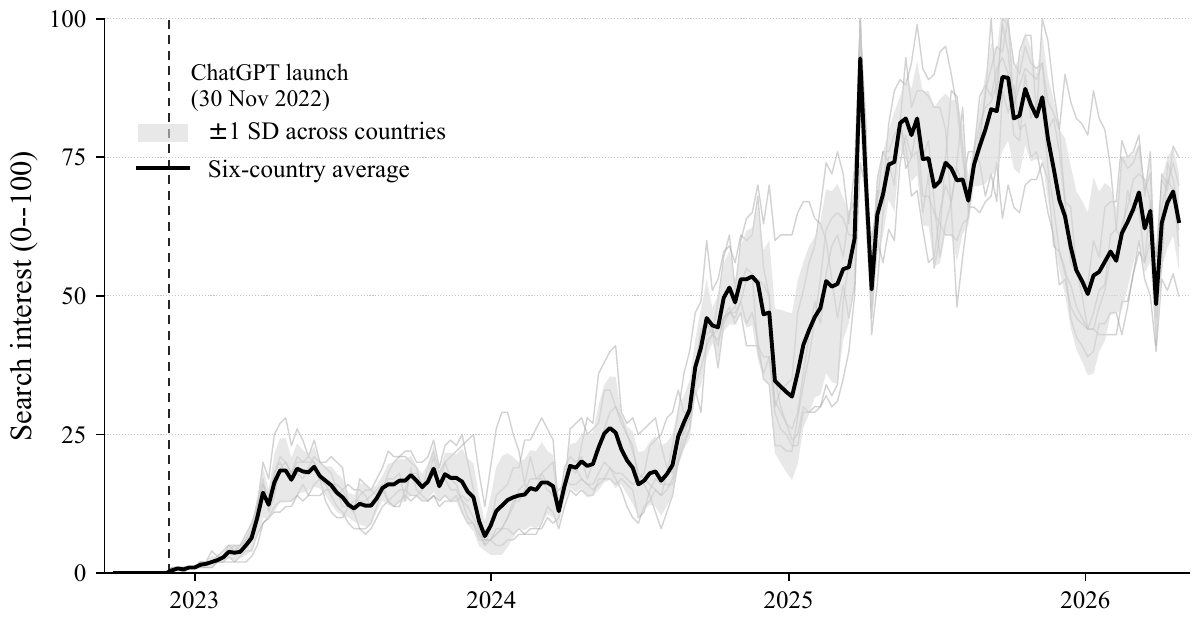
\includegraphics[width=\linewidth]{figures/fig_chatgpt_intro.png}

\column{0.43\linewidth}
\vspace{0.4em}
\small
\textbf{Interés de búsqueda en Google Trends} (CR, CO, EC, MX, PE, UY).
\vspace{0.4em}
\begin{itemize}\setlength\itemsep{0.25em}
  \item Línea base $\approx 0$ las 8 semanas previas al lanzamiento.
  \item Subida abrupta durante 2023.
  \item Máximo a inicios de 2025.
\end{itemize}
\vspace{0.6em}
{\color{pblue}\rule{\linewidth}{0.5pt}}
\vspace{0.4em}

\textbf{Reconocimiento $\neq$ adopción $\neq$ efecto causal} sobre el mercado laboral.
\end{columns}
\end{frame}

% ----- Por qué LatAm -----
\begin{frame}{¿Por qué América Latina?}
\vspace{0.3em}
\begin{itemize}
  \item \textbf{Informalidad estructural.} Tasa agregada $\approx 55\%$. Rango: $\sim 25\%$ Uruguay $\to >70\%$ región andina.
  \item \textbf{Mercados segmentados.} Formales e informales tienen instituciones distintas de fijación salarial, exposición digital y colchones frente a shocks de productividad.
  \item \textbf{Exposición estructuralmente distinta.} Azuara et al. \cit{BID 2024}: la exposición a LLMs se inclina hacia trabajadores formales, urbanos y con educación terciaria.
  \item \textbf{Lo que falta:} ningún artículo provee una \emph{estimación causal} de si esa exposición movió los resultados realizados del mercado laboral.
\end{itemize}

\vspace{0.4em}
\callout{La literatura latinoamericana existente \cit{Ciaschi et al.\ 2025; Egana-delSol \& Bravo-Ortega 2025} es \textbf{descriptiva sobre exposición}.}
\end{frame}

% ----- Research question + contribuciones -----
\begin{frame}{Pregunta de investigación y contribuciones}
\textbf{Pregunta.} ¿Cuál es el efecto causal de la exposición ocupacional a LLMs sobre empleo, salarios y horas en seis países de América Latina, y cómo varía con la formalidad de línea base?

\vspace{0.5em}
\textbf{Cinco contribuciones.}
\begin{enumerate}
  \item \textbf{Primeras estimaciones causales} no OCDE sobre el efecto laboral de los LLMs.
  \item Aplicación del \textbf{DiD con tratamiento continuo} de Callaway et al. \cit{2024} cada país.
  \item \textbf{Formalidad de línea base} como margen central de heterogeneidad intra-país. % (no como subgrupo de robustez)
  \item \textbf{Crosswalk y base armonizada} para 6 países (2021Q1--2025Q4), reproducible.
  \item \textbf{Cuatro narrativas pre-registradas}: el patrón por país queda determinado por el dato, no por búsqueda \emph{ex post} de especificación.
\end{enumerate}
\end{frame}

% ----- Marco teórico -----
\begin{frame}{Marco teórico estilizado: tareas, desplazamiento, reposición}
\vspace{0.2em}
{\color{cyan!30!blue!90!black}\textbf{Task-based production}} \cit{Acemoglu \& Autor 2011; Acemoglu \& Restrepo 2018, 2022}.
\vspace{0.3em}

Ocupación $o$ = paquete de tareas con shares $\{s_{oj}\}$. Exposición complementaria de Eloundou:
\[
\beta_o \equiv \sum_{j \in J^{\text{LLM}}} s_{oj}
\]
Respuesta salarial neta a la llegada de los LLMs:
\[
\Delta w_o = \underbrace{(\tau_r - \tau_d)}_{\text{reposición $-$ desplazamiento}} \cdot \beta_o
\]
\vspace{-0.4em}
\begin{itemize}
  \item Signo de $\tau_r - \tau_d$: \textbf{objeto empírico}, no predicción teórica.
  \item \textbf{Canal de la formalidad:} adopción requiere inversión de costo fijo $\Rightarrow$ se concentra en firmas formales. Por simetría, $\tau^F$ y $\tau^I$ pueden diferir en signo y magnitud.
\end{itemize}
\end{frame}

% ----- Cuatro narrativas preregistradas -----
\begin{frame}{Cuatro narrativas pre-registradas, evaluadas país por país}
\small
\vspace{0.1em}
\begin{tabularx}{\linewidth}{@{}p{3.4cm}X@{}}
\toprule
\textbf{Narrativa} & \textbf{Predicción para el país $c$} \\
\midrule
\textbf{A.} Informalidad amplifica & $|\hat\tau^c| > 2\%$ y $\tau^c_I < \tau^c_F < 0$. Los informales absorben más el shock. \\[0.3em]
\textbf{B.} Replicación del nulo & $|\hat\tau^c|$ pequeño y nulo en ambos canales. Perú/ALC = \cit{HV 2025a}. \\[0.3em]
\textbf{C.} Nulo formal, grande informal & $\tau^c_F \approx 0$ y $\tau^c_I$ significativamente negativo. Canal que DK/EE.UU.\ no pueden detectar. \\[0.3em]
\textbf{D.} Ganancias estratificadas & $\tau^c > 0$ sobre salarios, concentrado en formales urbanos con educación terciaria. \\
\bottomrule
\end{tabularx}

\vspace{0.7em}
\callout{Precomprometer las narrativas \textbf{antes} de mirar el dato post-tratamiento es la contribución metodológica del diseño. Las estimaciones de Perú se ejecutaron antes del depósito formal y se identifican como \textbf{exploratorias} en el mapeo a narrativas.}
\end{frame}

% ----- Estrategia empírica -----
\begin{frame}{Estrategia empírica: DiD continuo, país por país}
\small
\vspace{0.1em}
Una sola fecha global de adopción: $t^*=2022\text{Q4}$ (descartada como buffer; tratamiento efectivo desde 2023Q1).

\vspace{0.3em}
\textbf{Especificación primaria} (dentro del país $c$):
\vspace{-0.4em}
\[
Y^c_{ot} = \tau^c \cdot (\beta_o \cdot \text{Post}_t) + \alpha^c_o + \alpha^c_t + \varepsilon^c_{ot}.
\]

\vspace{-0.2em}
\begin{itemize}
  \item $Y^c_{ot}\in\{\log\text{empleo},\ \log\text{salario hora},\ \text{horas semanales}\}$ a nivel celda (ocupación, trimestre).
  \item $\beta_o$: exposición complementaria de Eloundou et al.\ \cit{2024}, mapeada a CIUO-08 4d (98.2\% match).
  \item Estimador continuo de Callaway, Goodman-Bacon \& Sant'Anna \cit{2024}; cohorte única $\Rightarrow$ TWFE ponderado.
  \item Errores agrupados a nivel ocupación CIUO-08 4d \cit{Abadie et al.\ 2023}.
  \item Soporte: \emph{event study} Sun--Abraham, binario CS-2021 en la mediana, shift-share, \emph{wild cluster bootstrap}.
\end{itemize}
\end{frame}

% ----- Datos: armonización -----
\begin{frame}{Datos: armonización a CIUO-08 4d en seis países}
\footnotesize
\vspace{0.2em}
\begin{tabularx}{\linewidth}{@{}llXX@{}}
\toprule
\textbf{País} & \textbf{Encuesta} & \textbf{Frecuencia} & \textbf{Armonización}\\
\midrule
Costa Rica & ECE     & Trimestral             & CIUO-08 4d directo \\
Colombia   & GEIH    & Mensual                & Agregar 3 meses $\to$ trimestre \\
Ecuador    & ENEMDU  & Mensual (continua)     & Agregar 3 meses $\to$ trimestre \\
México   & ENOE    & Trimestral             & SINCO $\to$ CIUO-08 (INEGI, 97.4\%) \\
\textbf{Perú} & \textbf{EPEN} & \textbf{Trimestral, solo Lima Metro} & \textbf{CO1995 $\to$ CNO2015 $\to$ CIUO08} \\
Uruguay    & ECH     & Anual (campo continuo) & Separar por mes de entrevista \\
\bottomrule
\end{tabularx}

\vspace{0.6em}
\normalsize
\begin{itemize}
  \item Ventana común: \textbf{2021Q1--2025Q4} (post-COVID estricto).
  \item \textbf{Pre} corto: 7 trimestres limpios. Se compensa con cotas Honest-DiD \cit{Rambachan \& Roth 2023}.
\end{itemize}
\end{frame}

% ----- Peru: clasificador -----
\begin{frame}{Perú: el cambio de clasificador coincide con el shock}
\small
\vspace{0.1em}
\textbf{Reto técnico central.} La EPEN cambió el clasificador ocupacional \textbf{en 2022Q4}:
\begin{itemize}
  \item 2021Q1--2022Q3: CO-1995 a 3 dígitos (319 códigos).
  \item 2022Q4--2025Q4: CNO-2015 a 4 dígitos (473 códigos).
  \item \textbf{El corte cae en la misma fecha de tratamiento.}
\end{itemize}

\vspace{0.4em}
\textbf{Solución.} Llevar ambos períodos a CIUO-08 4d vía los cuatro Anexos del INEI, con \textbf{pesos posteriores empíricos} condicionales en $(k, \text{sexo}, \text{educ}, \text{ISIC}, \text{dominio})$ estimados sobre el post.

\vspace{0.4em}
\textbf{Validación (pre-registrada).}
\begin{itemize}
  \item Salto máximo de \emph{shares} CIUO entre 2022Q3 y 2022Q4: \textbf{2.05 p.p.} (umbral $\leq 5$ p.p.). $\checkmark$
  \item Divergencia KL máxima de los pesos entre 2023--2025: \textbf{0.046 nats} (umbral $\leq 0.05$). $\checkmark$
  \item \emph{Donut} DiD descartando 2022Q3--Q4: por reportar en robustez.
\end{itemize}
\end{frame}

% ----- Descriptivos Peru -----
\begin{frame}{Lima Metropolitana 2021: descriptivos}
\vspace{0.2em}
\begin{columns}[T,onlytextwidth]
\column{0.50\linewidth}
\footnotesize
\textbf{Composición de la muestra (2021):}
\begin{itemize}\setlength\itemsep{0.25em}
  \item Edad media 37.7 (DE 12.5)
  \item \% mujeres: 44.9\%
  \item \% terciaria/postsec.: 36.3\%
  \item \% formal (`seguro1' $\in\{1,3\}$): 36.7\%
  \item Horas semanales: 43.4
  \item $\log$ salario/hora: 1.88
\end{itemize}

\vspace{0.5em}
\textbf{Exposición $\beta$ ponderada por empleo:}
\begin{itemize}\setlength\itemsep{0.20em}
  \item Media 0.280, DE 0.178
  \item $p_{50}=0.255$,\ $p_{90}=0.503$
  \item \textbf{25.6\%} de trabajadores con $\beta=0$
  \item Formalidad sube de 25.8\% (Q1) a 50.6\% (Q4 de $\beta$)
\end{itemize}

\column{0.48\linewidth}
\centering
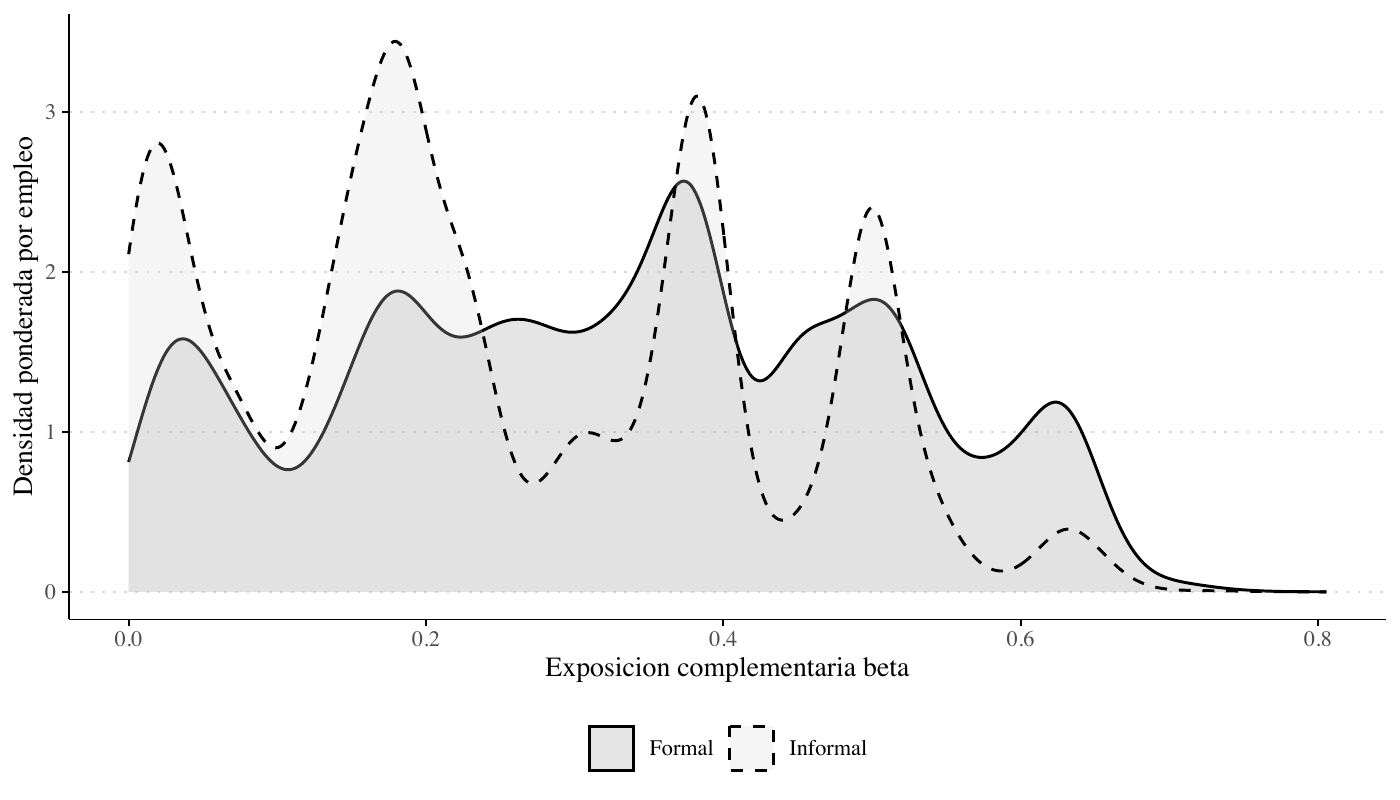
\includegraphics[width=\linewidth]{figures/fig_peru_beta_dist.png}

\vspace{0.2em}
{\footnotesize\color{pgray}Densidad de $\beta$ por formalidad de línea base.}
\end{columns}
\end{frame}

% ----- Resultados agregados -----
\begin{frame}{Resultado 1: estimaciones agregadas para Perú}
\vspace{0.1em}
\footnotesize
\renewcommand{\arraystretch}{1.05}
\begin{tabularx}{\linewidth}{@{}lCCC@{}}
\toprule
 & $\log$ empleo & $\log$ salario/hora & Horas semanales \\
\midrule
\multicolumn{4}{@{}l}{\itshape Panel A. TWFE continuo (especificación principal)}\\
$\hat\tau^{\text{Perú}}$ & 0.221 & 0.042 & $-3.250$ \\
                            & (0.220) & (0.062) & (1.852) \\
$p$-valor                   & 0.317 & 0.498 & 0.082 \\
\midrule
\multicolumn{4}{@{}l}{\itshape Panel B. Callaway--Sant'Anna binario (corte en la mediana ponderada 2021), balanced}\\
$\hat\tau^{\text{Perú, bin}}$ & \textbf{0.144}$^{***}$ & 0.006 & $\bm{-0.801}^{**}$ \\
                                 & (0.025) & (0.011) & (0.333) \\
IC 95\%                          & [0.095, 0.192] & [$-$0.016, 0.029] & [$-$1.454, $-$0.148] \\
\midrule
$N$ celdas & 2,139 & 2,139 & 2,139 \\
$N$ códigos CIUO & \multicolumn{3}{l}{138 (Panel A) / 67 (Panel B, balanceado)}\\
\bottomrule
\end{tabularx}

\vspace{0.4em}
\footnotesize
\begin{itemize}\setlength\itemsep{0.15em}
  \item \textbf{Panel A:} en aislamiento, sugiere \emph{replicación del nulo} \cit{HV 2025a}.
  \item \textbf{Panel B:} con agregación correcta de los ATT$(g,t)$, aparece efecto \emph{positivo} sobre empleo y \emph{negativo} sobre horas.
\end{itemize}
\end{frame}

% ----- Honest-DiD weakness -----
\begin{frame}{Robustez 1: cota Honest-DiD}
\small
\vspace{0.1em}
\textbf{Criterio pre-registrado.} Las afirmaciones principales requieren un valor de quiebre $\bar{M}^c \geq 2$ \cit{Rambachan \& Roth 2023}.

\vspace{0.4em}
\textbf{Resultado para Perú (Panel A).} Para los tres \emph{outcomes}, $\bar{M}^{\text{Perú}} = 0$: el IC 95\% original \textbf{ya incluye cero}, por lo que el criterio de quiebre no separa la especificación continua de la hipótesis nula.

\vspace{0.4em}
\weak{La especificación continua TWFE \textbf{no supera el estándar de robustez que el propio artículo se impuso}. Reporto el resultado de manera transparente. A la luz de esto, el binario Callaway--Sant'Anna (Panel B) se trata como la \textbf{lectura preferida del agregado}.}

\vspace{0.3em}
\callout[pgray]{La discrepancia es informativa: en presencia de respuestas heterogéneas a la dosis, los pesos implícitos del TWFE pueden ser negativos y diluir el promedio \cit{de Chaisemartin \& D'Haultfœuille 2020; Sun \& Abraham 2021}.}
\end{frame}

% ----- Tendencias paralelas -----
\begin{frame}{Resultado 2: tendencias previas y dinámica del efecto}
\vspace{0.2em}
\begin{columns}[T,onlytextwidth]
\column{0.46\linewidth}
\centering
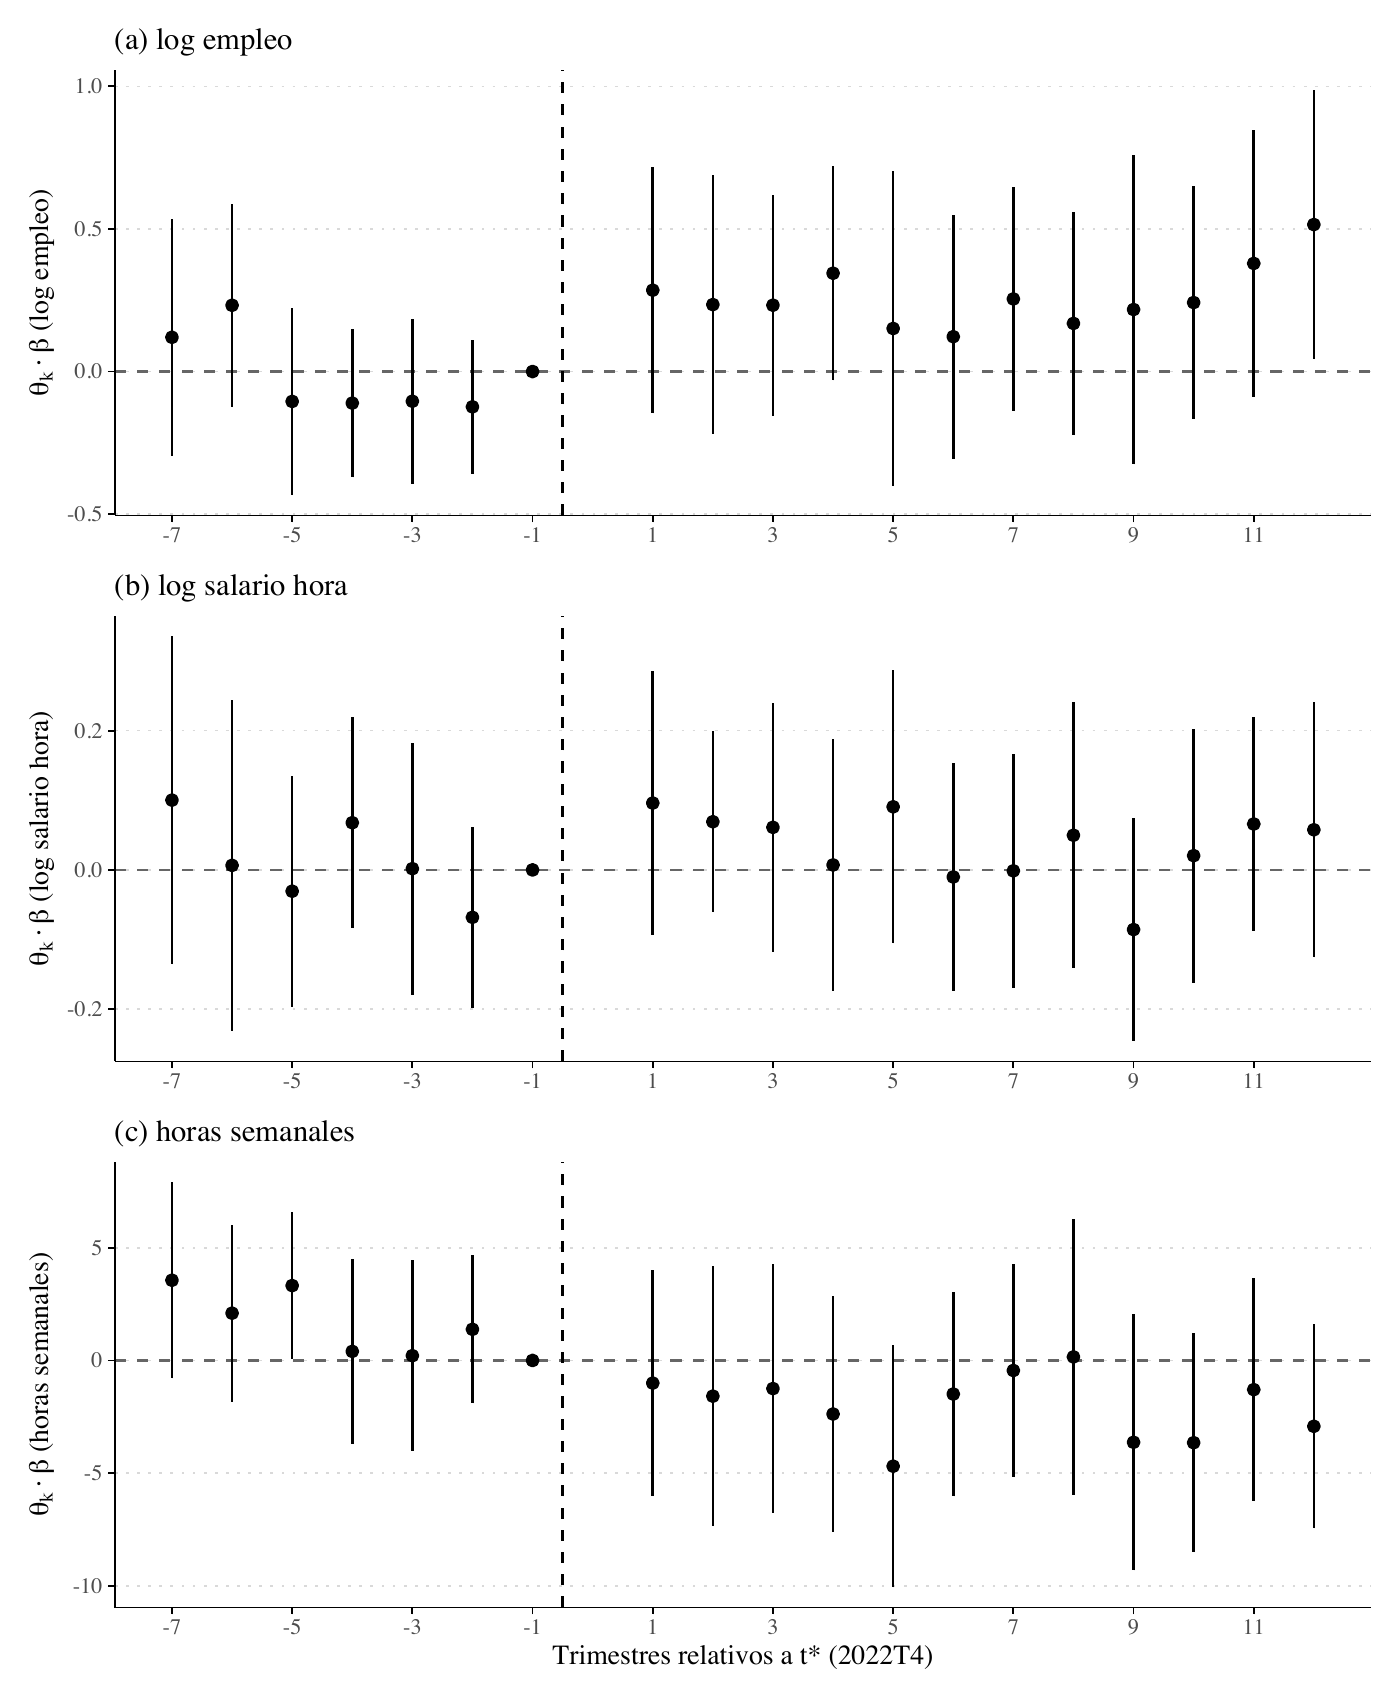
\includegraphics[height=0.78\textheight,keepaspectratio]{figures/fig_peru_event_study.png}

\column{0.51\linewidth}
\footnotesize
\textbf{Test conjunto de Wald, $k\in[-7,-2]$:}
\begin{itemize}\setlength\itemsep{0.15em}
  \item $\log$ empleo: $F=1.534$ ($p=0.171$)
  \item $\log$ salario/hora: $F=1.298$ ($p=0.262$)
  \item Horas: $F=1.515$ ($p=0.178$)
\end{itemize}

\vspace{0.5em}
\textbf{Empleo (panel a).} Los 12 coeficientes post son \emph{positivos sin excepción}, de $+0.25$ a $+0.52$.

\vspace{0.4em}
\textbf{Horas (panel c).} Pre-coeficientes sistemáticamente positivos, post negativos.

\vspace{0.5em}
\weak{El perfil de \emph{inversión} en horas sugiere una posible reversión de tendencia que podría inflar mecánicamente el coeficiente principal. Sigo a Roth \cit{2022} en pesarlo con cautela.}
\end{columns}
\end{frame}

% ----- Heterogeneidad por formalidad -----
\begin{frame}{Resultado 3: heterogeneidad por formalidad de línea base}
\vspace{0.1em}
\footnotesize
\renewcommand{\arraystretch}{1.15}
\begin{tabularx}{\linewidth}{@{}lCCC@{}}
\toprule
 & $\log$ empleo & $\log$ salario/hora & Horas semanales \\
\midrule
$\hat\tau^{\text{Perú}}_F$ (canal formal)
   & \textbf{0.567}$^{***}$ & $\bm{-0.128}^{**}$ & $-1.920^{*}$ \\
   & (0.211) & (0.056) & (1.034) \\
$\hat\tau^{\text{Perú}}_I$ (canal informal)
   & $-0.222$ & \textbf{0.265}$^{***}$ & $-5.110$ \\
   & (0.286) & (0.080) & (3.819) \\
\midrule
$\hat\tau_F - \hat\tau_I$ & 0.790 & $-0.394$ & 3.190 \\
$z$-stat                  & 2.80  & $-4.19$  & 0.82 \\
$p$-valor (igualdad)      & \textbf{0.005} & \textbf{$<$0.001} & 0.410 \\
\bottomrule
\end{tabularx}

\vspace{0.4em}
\normalsize
\callout{El cuadro empírico contradice la lectura agregada del nulo. Canal formal y canal informal se mueven en \textbf{direcciones opuestas} y estadísticamente significativas en dos de los tres \emph{outcomes}. \textbf{El nulo agregado es un artefacto de cancelación.}}
\end{frame}

% ----- Heterogeneidad: visual -----
\begin{frame}{Heterogeneidad por formalidad: visualización}
\centering
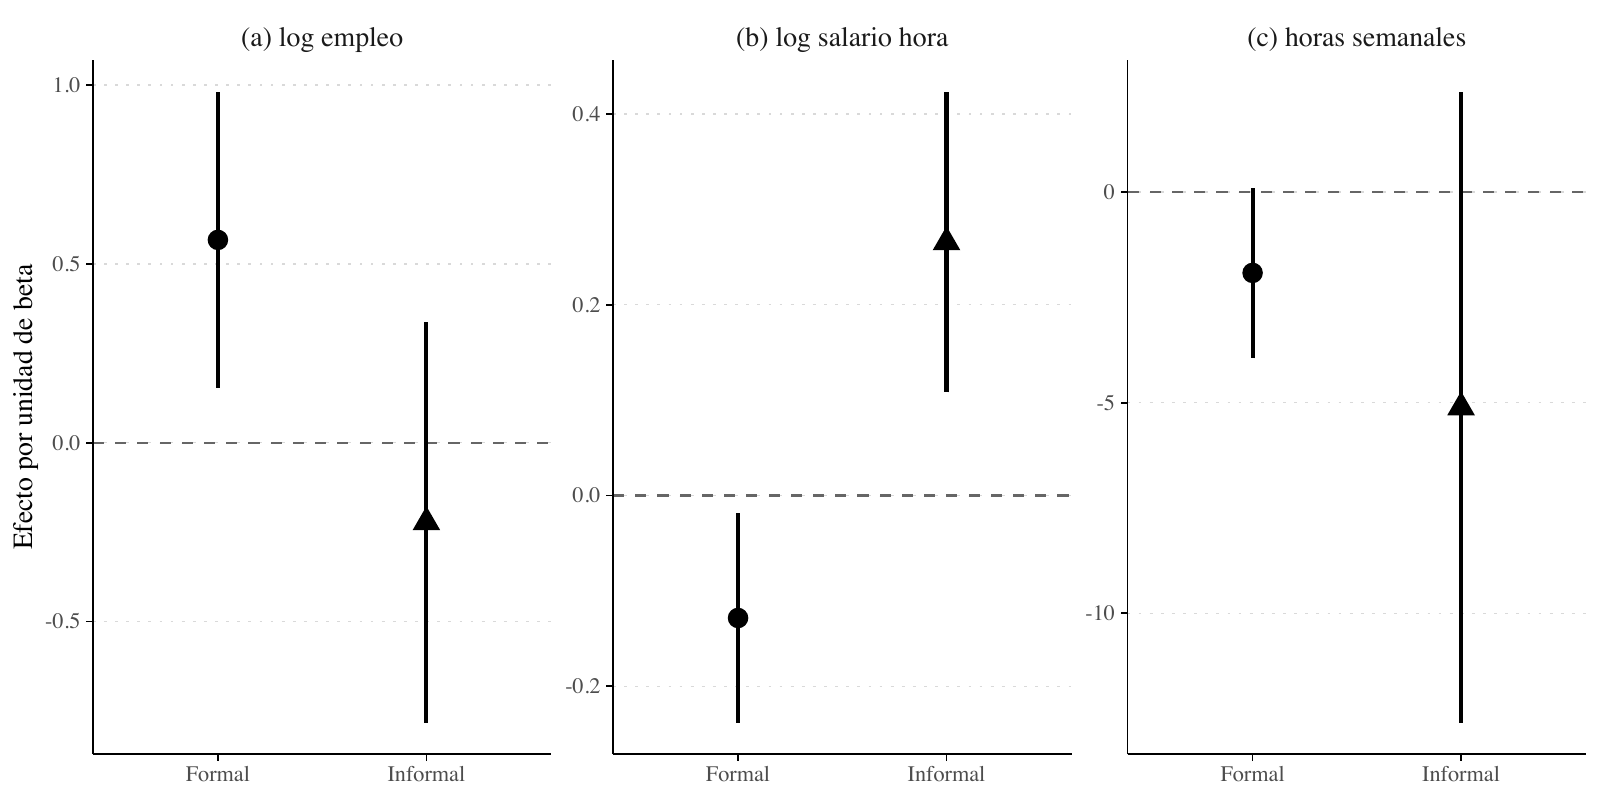
\includegraphics[height=0.72\textheight,keepaspectratio]{figures/fig_peru_formality.png}

\vspace{0.3em}
{\footnotesize\color{pgray}%
Coeficientes $\hat\tau_F$ (canal formal) y $\hat\tau_I$ (canal informal) con IC 95\%. Diferencia significativa para empleo ($p=0.005$) y salario/hora ($p<0.001$).%
}
\end{frame}

% ----- Síntesis Peru -----
\begin{frame}{Síntesis: el \textquotedblleft Patrón Peruano\textquotedblright\ emergente}
\footnotesize
\vspace{0.1em}
\textbf{Honesto sobre el mapeo a narrativas.} Ninguna de las cuatro pre-registradas reproduce exactamente el patrón de Lima.

\vspace{0.3em}
\begin{itemize}\setlength\itemsep{0.10em}
  \item A: requería $\tau_F < 0$ -- pero $\hat\tau_F^{\text{empleo}}>0$.
  \item B: requería ambos canales nulos -- rechazo de igualdad en empleo y salario.
  \item C: requería $\tau_F\approx 0$ -- magnitud y significancia del canal formal lo contradicen.
  \item D: predecía ganancias salariales en formales -- el signo \emph{salarial} formal es \textbf{opuesto}.
\end{itemize}

\vspace{0.3em}
\callout{\textbf{Patrón Peruano (exploratorio).} Las ocupaciones formales-dominantes expuestas a LLMs \emph{expanden empleo} y \emph{reducen horas}, con presión bajista sobre salario/hora. Las informales-dominantes exhiben \emph{contracción débil de empleo} con salarios al alza entre los presentes en la ocupación (selección positiva o equilibrio general).}

\vspace{0.2em}
{\normalsize\textbf{Quinto patrón} a añadir a la pre-registración formal antes de mirar el dato post de los cinco países restantes.}
\end{frame}

% ----- Puntos débiles (I): identificación y datos -----
\begin{frame}{Puntos a considerar (I): identificación y datos}
\footnotesize
\vspace{0.2em}
\begin{enumerate}\setlength\itemsep{0.35em}
  \item \textbf{Cobertura geográfica.} La EPEN cubre sólo Lima Metropolitana. $\hat\tau^{\text{Perú}}$ no es nacionalmente representativo. Validación prevista con ENAHO anual.
  \item \textbf{Definición de formalidad.} Basada en `seguro1' (afiliación a ESSALUD). La definición OIT (pensiones) requiere ENAHO.
  \item \textbf{Honest-DiD $= 0$ en el TWFE continuo.} La especificación principal \textbf{no supera} el criterio de robustez pre-registrado ($\bar{M}\geq 2$). La lectura preferida pasa al binario Callaway--Sant'Anna.
  \item \textbf{Reversión de tendencia en horas.} Pre-coeficientes positivos en el \emph{event study}; podría inflar el coeficiente principal de horas \cit{Roth 2022}.
\end{enumerate}
\end{frame}

% ----- Puntos débiles (II): supuestos y método -----
\begin{frame}{Puntos a considerar (II): supuestos y método}
\footnotesize
\vspace{0.2em}
\begin{enumerate}\setlength\itemsep{0.35em}
  \setcounter{enumi}{4}
  \item \textbf{Selección no modelada.} EPEN es corte transversal repetido. Migración ocupacional, salida al desempleo y recomposición demográfica no son identificables aquí.
  \item \textbf{Crosswalk descansa en pesos posteriores empíricos.} Pendiente: escalera completa de robustez (CO-1995 3d, \emph{donut} DiD, pesos uniformes, solo-post).
  \item \textbf{SUTVA.} Derrames intra-firma sesgan hacia cero el desplazamiento estimado; la cota narrativa \cit{Berg et al.\ 2018} acota la magnitud pero no la elimina.
  \item \textbf{Pre-período corto.} Solo 7 trimestres entre 2021Q1 y 2022Q3. Las pruebas de tendencias previas tienen poco poder.
  \item \textbf{Las estimaciones de Perú son pre-depósito.} Se identifican como \emph{exploratorias} en el mapeo a narrativas; el pre-registro formal en OSF cubrirá los 5 países restantes.
\end{enumerate}
\end{frame}

% ----- Próximos pasos -----
\begin{frame}{Próximos pasos}
\small
\vspace{0.1em}
%\textbf{Corto plazo}
\begin{itemize}
  \item Cerrar escalera de robustez del clasificador para Perú (5 columnas).
  \item Validar con ENAHO anual nacional (representatividad + definición OIT de formalidad).
  \item Reportar medidas alternativas de exposición: $\alpha$, $\zeta$ \cit{Eloundou et al.\ 2024}; Webb \cit{2019}; AIOE \cit{Felten et al.\ 2021}.
  \item Cotas Honest-DiD, Oster \cit{2019}, shift-share con SE de Adão--Kolesár--Morales.
%\end{itemize}

\vspace{0.3em}
%\textbf{Mediano plazo.}
%\begin{itemize}
  \item Replicar el \emph{pipeline} en Costa Rica, Colombia, Ecuador, México, Uruguay.
  %\item Pre-registro formal en OSF para los 5 países restantes, incluyendo el \emph{Patrón Peruano} como hipótesis adicional.
  \item Comparación lado a lado de los seis $\{\hat\tau^c\}_{c=1}^{6}$: contribución empírica central.
%\end{itemize}

%\vspace{0.3em}
%\textbf{Largo plazo.}
%\begin{itemize}
  %\item Segundo artículo: panel rotativo de la ENOE de México para estimar \emph{transiciones individuales} entre ocupaciones de distinta exposición.
\end{itemize}
\end{frame}

% ----- Referencias clave -----
\begin{frame}{Algunas referencias clave}
\scriptsize
\setlength{\parskip}{0.30em}

Acemoglu, D. \& Restrepo, P. (2022). Tasks, Automation, and the Rise in U.S. Wage Inequality. \emph{Econometrica} 90(5).

Azuara Herrera, O., Ripani, L. \& Torres Ramírez, E. (2024). \emph{AI and the Increase of Productivity and Labor Inequality in Latin America}. BID.

Callaway, B., Goodman-Bacon, A. \& Sant'Anna, P.H.C. (2024). \emph{Difference-in-Differences with a Continuous Treatment}. NBER WP 32117.

Callaway, B. \& Sant'Anna, P.H.C. (2021). DiD with Multiple Time Periods. \emph{J. Econometrics} 225(2).

Chen, D. et al. (2025). \emph{The (Short-Term) Effects of LLMs on Unemployment and Earnings}.

Ciaschi, M. et al. (2025). \emph{Potential Distributive Impact of AI-Driven Labor Changes in LAC}. BID.

Egana-delSol, P. \& Bravo-Ortega, C. (2025). \emph{AI and Labor Market Transformations in Latin America}. IZA DP 17746.

Eloundou, T., Manning, S., Mishkin, P. \& Rock, D. (2024). GPTs Are GPTs. \emph{Science} 384(6702).

Hartley, J. et al. (2024). \emph{The Labor Market Effects of Generative AI}. SSRN WP.

Humlum, A. \& Vestergaard, E. (2025a). \emph{Large Language Models, Small Labor Market Effects}. BFI WP 2025-56.

Rambachan, A. \& Roth, J. (2023). A More Credible Approach to Parallel Trends. \emph{Rev. Econ. Stud.} 90(5).

Roth, J. (2022). Pretest with Caution. \emph{AER: Insights} 4(3).

Sun, L. \& Abraham, S. (2021). Estimating Dynamic Treatment Effects in Event Studies. \emph{J. Econometrics} 225(2).
\end{frame}

% ----- Cierre -----

\end{document}
